\documentclass[9pt,conference]{IEEEtran}
\usepackage{cite}
\usepackage{amsmath,amssymb,amsfonts}
\usepackage{multirow}
\usepackage{array}
\usepackage{graphicx}
\usepackage{textcomp}
\usepackage{xcolor}
\usepackage{algorithm}
\usepackage[noend]{algpseudocode}
\usepackage{hhline}
\usepackage{mathrsfs}
\usepackage{float}
\graphicspath{{Figures/}}
\usepackage{epstopdf}
\epstopdfsetup{outdir=./}

\begin{document}

\title{GROUP\_14\_Experiment: 3\\Characterization of CMOS Inverter}

\author{
    \IEEEauthorblockA{Siddhant Shah (B23334) *, Akash Goel(B23032) †, 
                      Om Maheshwari (B23089) ‡, and Somya Bhadada (B23052) §}
* b23334@students.iitmandi.ac.in \\
† b23032@students.iitmandi.ac.in \\
‡ b23089@students.iitmandi.ac.in \\
§ b23052@students.iitmandi.ac.in}
\date{}

\maketitle


\begin{abstract}
\noindent{CMOS Known as complementary symmetrical metal oxide semiconductor (COS-MOS) is combined effect of PMOS and NMOS with their duality nature.CMOS inverter is basically consider as nucleus of all VLSI circuits. This lab report represents a study of CMOS Inverter and its characteristics.}
\end{abstract}

\section{Components Required}
\begin{itemize}
\begin{itemize}
    \item CD4007 IC
    \item Digital Multimeter (DMM)
    \item Function Generator
    \item Digital Storage Oscilloscope (DSO)
    \item Power Supply
    \item Breadboard
    \item Connecting Wires
\end{itemize}
\end{itemize}

\section{Theory}
CMOS logic circuit has two planes in vertical manner:
\begin{enumerate}
    \item Array of PMOS,Which allows to charge load capacitance up to power supply.Also,combination/array of PMOS is defined as pull-up device.
    \item Array of NMOS,Which allows to discharge load capacitance up to power supply.ALSO, combination/array of NMOS is defined as pull-down device.
\end{enumerate}

\noindent{CMOS inverter is designed with single PMOS and NMOS with tied of both transistor's gate terminal with single input and ensure that biasing connection in reverse manner  respective to source and drain terminal of both transistors.}
\noindent{As shown in Fig.1, Working Principle Of CMOS Inverter With low input($V_{IL}$,Logic 0) and PMOS goes to on state with pull up to load capacitance to Vdd level(logic 1).}

\begin{figure}[H]
\centering
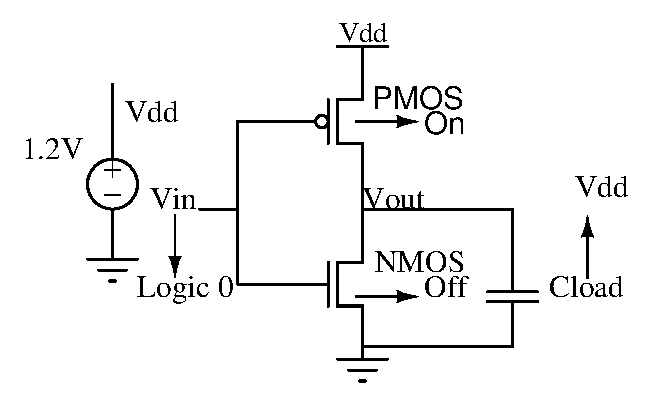
\includegraphics[width=0.3\textwidth]{CMOS.eps}
\caption{\label{fig:CMOS.eps}Charging load capacitance up to Vdd Level.}
\end{figure}
\noindent{In Similar to opposite apply of input high voltage($V_{IH}$,Logic 1),NMOS goes to on state with pull down to load capacitance to Gnd level(logic 0) as shown in fig.2.}\\

\begin{figure}
\centering
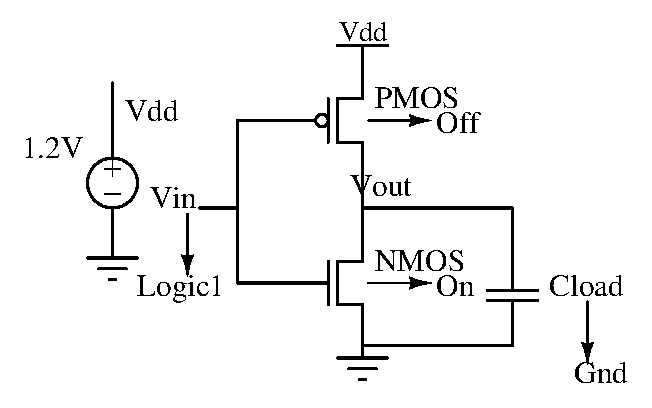
\includegraphics[width=0.3\textwidth]{CMOS2.eps}
\caption{\label{fig:CMOS2.eps}Discharging load capacitance up to  Level.}
\end{figure}\\

\begin{figure}[H]
    \centering
    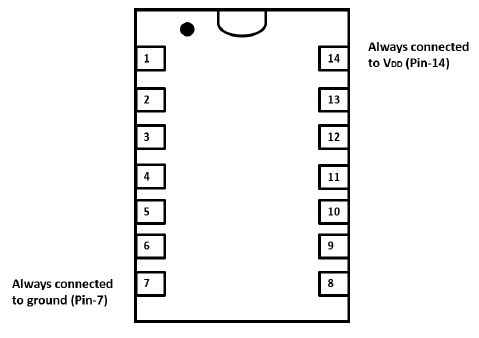
\includegraphics[width=0.7\columnwidth]{CD4007IC.png}
    \caption{CMOS Pin Diagram}
    \label{fig:clamper_circuit}
\end{figure}

\noindent{When a square wave is applied as the input to a CMOS inverter, the output undergoes transitions between logic high \((V_{dd})\) and logic low \((0V)\). These transitions introduce rise time, fall time, and propagation delay, which are critical in determining the performance of digital circuits.}\\

Rise Time (\( t_r \))
Definition:
\begin{itemize}
    \item Rise time \((t_r)\) is the time taken for the output voltage to transition from \(10\%\) to \(90\%\) of \( V_{dd} \).
    \item This occurs when the input transitions from HIGH to LOW, causing the PMOS transistor to turn ON and pull the output up to \( V_{dd} \).
\end{itemize}

Calculation:
\begin{equation}
    t_r \approx 2.2 \times R_p C_L
\end{equation}
where:
\begin{itemize}
    \item \( R_p \) is the PMOS transistor resistance.
    \item \( C_L \) is the load capacitance.\\
\end{itemize}


Fall Time (\( t_f \))
Definition:
\begin{itemize}
    \item Fall time \((t_f)\) is the time taken for the output voltage to transition from \(90\%\) to \(10\%\) of \( V_{dd} \).
    \item This occurs when the input transitions from LOW to HIGH, turning the NMOS transistor ON and pulling the output voltage to \( 0V \).
\end{itemize}
Calculation:
\begin{equation}
    t_f \approx 2.2 \times R_n C_L
\end{equation}
where:
\begin{itemize}
    \item \( R_n \) is the NMOS transistor resistance.
    \item \( C_L \) is the load capacitance.\\
\end{itemize}

Propagation Delay (\( t_p \))
Definition:
\noindent{Propagation delay is the time taken for the inverter to respond to an input transition.}\\

Types of Propagation Delay:
\begin{itemize}
    \item Low-to-High Delay \( t_{PLH} \)
    \begin{itemize}
        \item The time taken for the output to transition from LOW \((0V)\) to HIGH \((V_{dd})\) when the input goes from HIGH to LOW.
        \item Dominated by the PMOS transistor characteristics.
        \item Formula:
        \begin{equation}
            t_{PLH} \approx 0.69 \times R_p C_L
        \end{equation}
    \end{itemize}
    
    \item High-to-Low Delay \( t_{PHL} \)
    \begin{itemize}
        \item The time taken for the output to transition from HIGH \((V_{dd})\) to LOW \((0V)\) when the input goes from LOW to HIGH.
        \item Dominated by the NMOS transistor characteristics.
        \item Formula:
        \begin{equation}
            t_{PHL} \approx 0.69 \times R_n C_L
        \end{equation}
    \end{itemize}
\end{itemize}

Total Propagation Delay:
\begin{equation}
    t_p = \frac{t_{PLH} + t_{PHL}}{2}
\end{equation}
This represents the average delay in switching.

\noindent{When analyzing a CMOS inverter with a square wave input, we study:}
\begin{itemize}
    \item  Rise Time \( (t_r) \) – Time to rise from \(10\%\) to \(90\%\) of \( V_{dd} \).
    \item Fall Time \( (t_f) \) – Time to fall from \(90\%\) to \(10\%\) of \( V_{dd} \).
    \item Propagation Delay \( (t_p) \) – Average time for the output to respond to an input change.
\end{itemize}


\section{Observations and Results}
\begin{itemize}
    \item Implemented a CMOS Inverter Circuit on the breadboard same as the circuit which is given below
\end{itemize}
\begin{figure}[H]
    \centering
    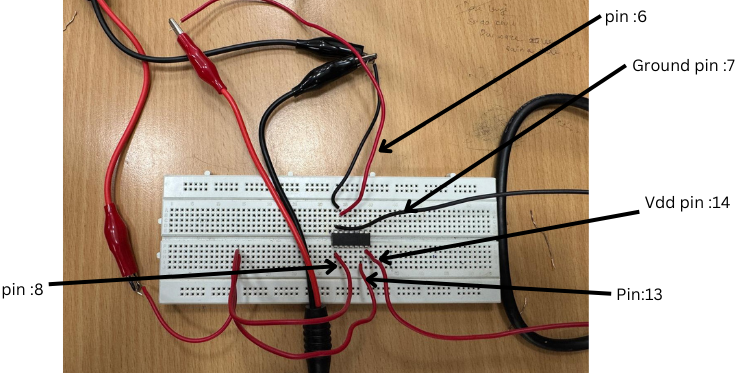
\includegraphics[width=1.0\columnwidth]{CMOS_Inverter_Circuit.png}
    \caption{CMOS Inverter Circuit}
    \label{fig:clamper_circuit}
\end{figure}

\begin{itemize}
    \item A CMOS inverter consists of a PMOS and NMOS transistor connected in a complementary configuration, with the input applied to both gates and the output taken from the common drain.
    \item The applied input is a ramp signal ranging from 0V to 5V with a 2.5V offset, ensuring it spans the full logic range.
    \item When the input voltage is low (close to 0V), the NMOS transistor is off, and the PMOS is fully on, resulting in the output being pulled up to Vdd (5V).
    \item As the input voltage increases, the NMOS transistor starts conducting, and the PMOS begins turning off, leading to a gradual drop in output voltage.
    \item When the input reaches 2.5V (midpoint of the ramp), both transistors are in the transition region, causing a rapid voltage change at the output due to high gain around the switching threshold.
    \item As the input voltage approaches 5V, the NMOS is fully on, and the PMOS is off, pulling the output down to 0V.
    \item The output waveform is an inverted version of the input ramp, transitioning sharply around the threshold voltage.
    \item This behavior is evident in the voltage transfer characteristic (VTC) curve, where the output exhibits a steep transition between logic states.
\end{itemize}

\begin{figure}[H]
    \centering
    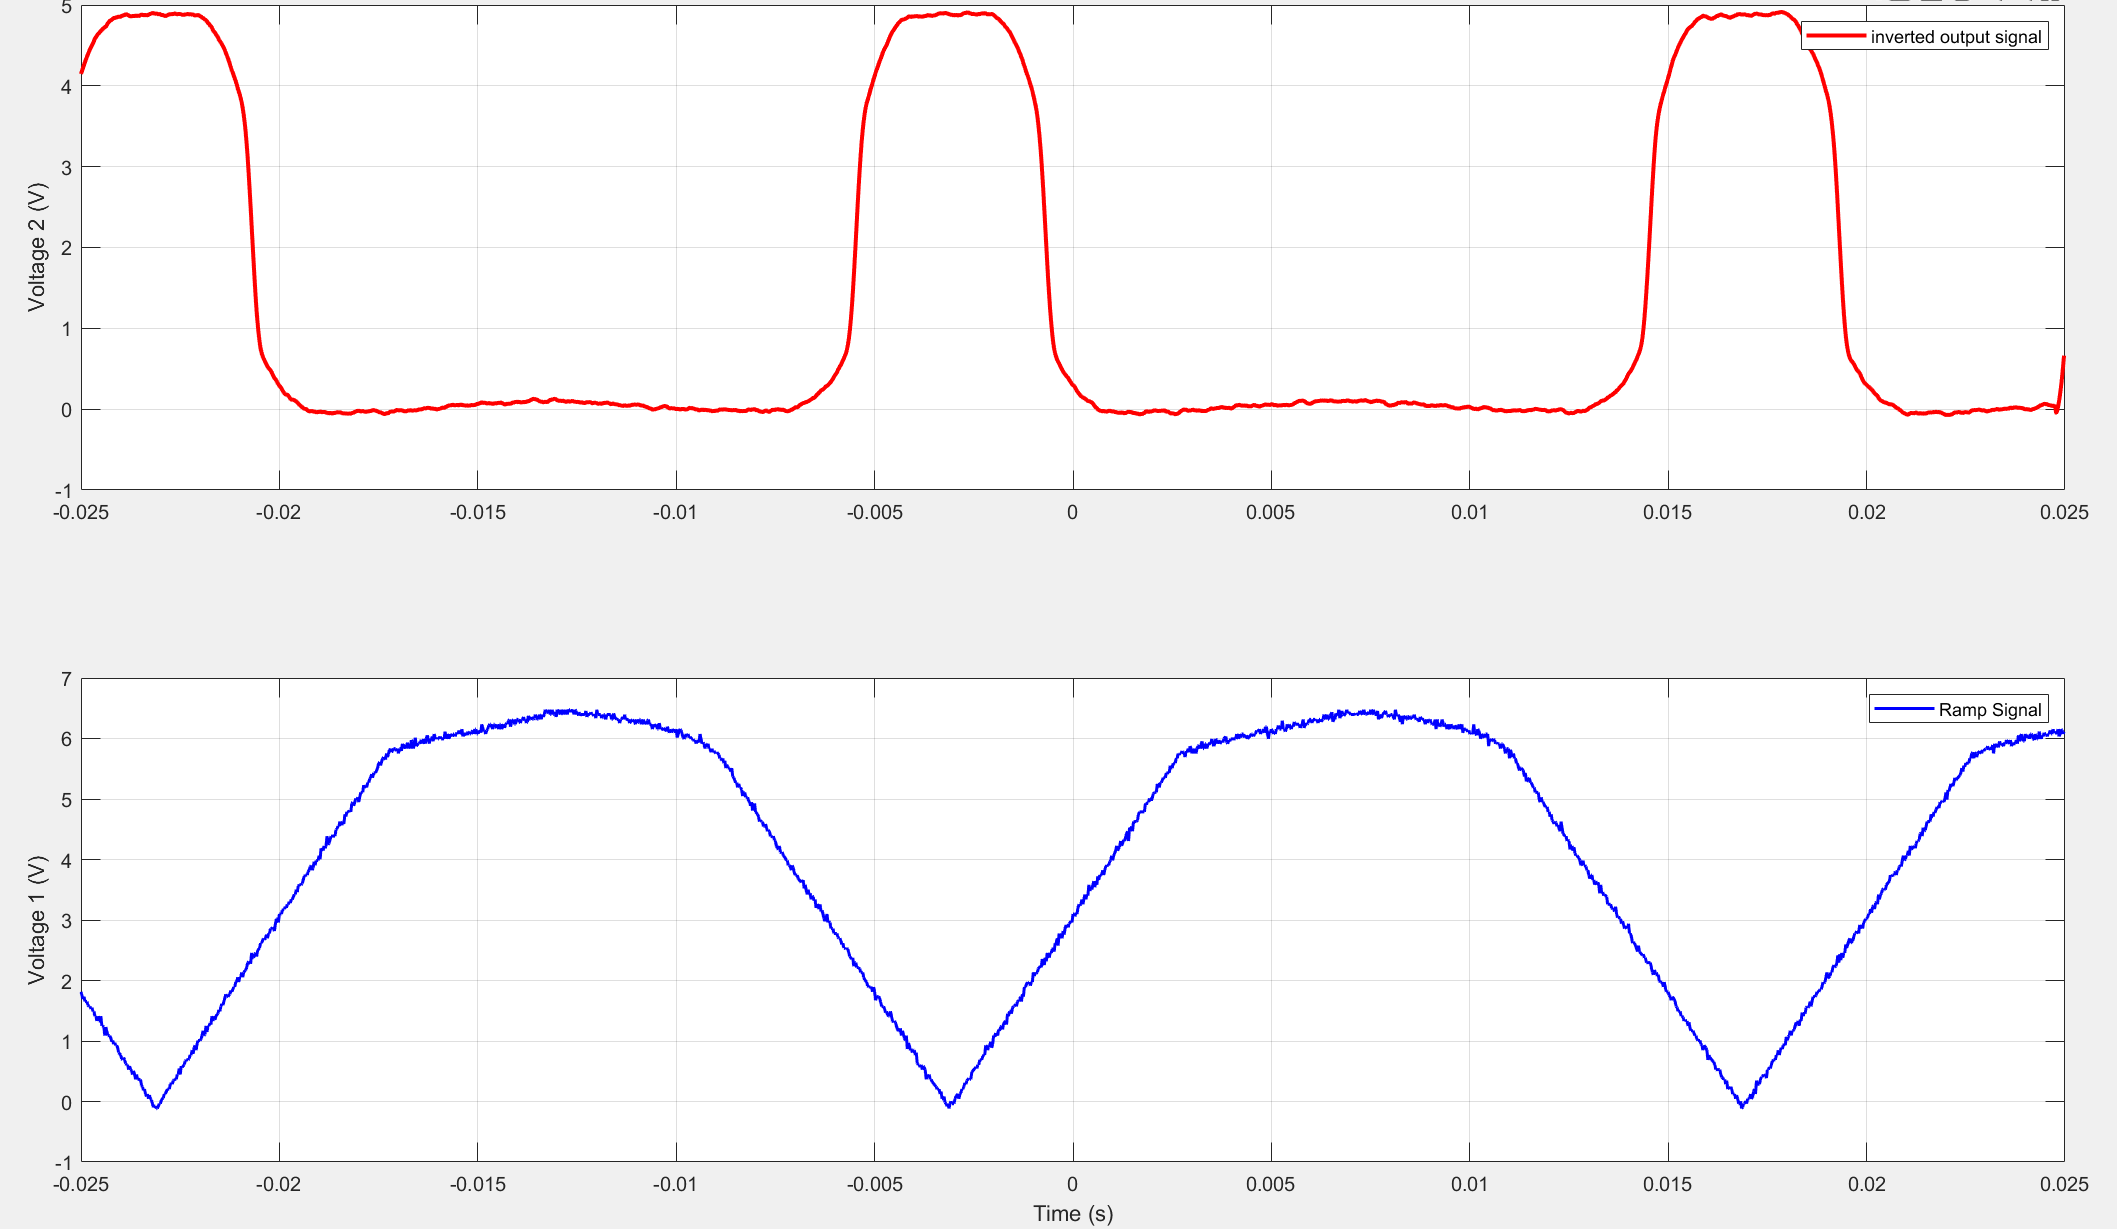
\includegraphics[width=1.0\columnwidth]{CMOS_Inverter_Circuit_graph.png}
    \caption{CMOS Inverter Circuit graph}
    \label{fig:clamper_circuit}
\end{figure}

\begin{itemize}
    \item Now if we compare to the LTspice results , you can see the circuit and the graph below . The results which we obtain on LTspice exactly match our Lab output. Hence, The circuit is verified.
\end{itemize}
\begin{figure}[H]
    \centering
    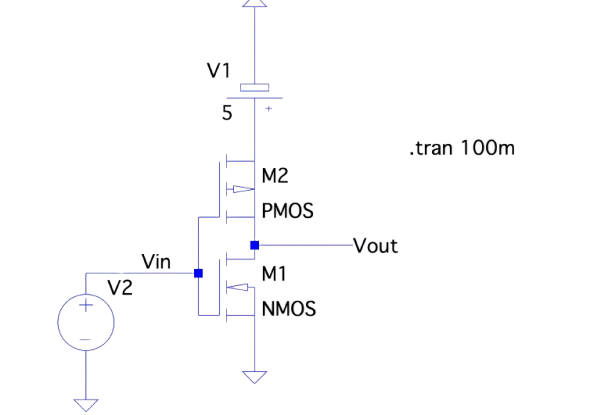
\includegraphics[width=1.0\columnwidth]{LTspice_CMOS_Inverter.png}
    \caption{LTspice CMOS Inverter Circuit}
    \label{fig:positive_clamper}
\end{figure}
\begin{figure}[H]
    \centering
    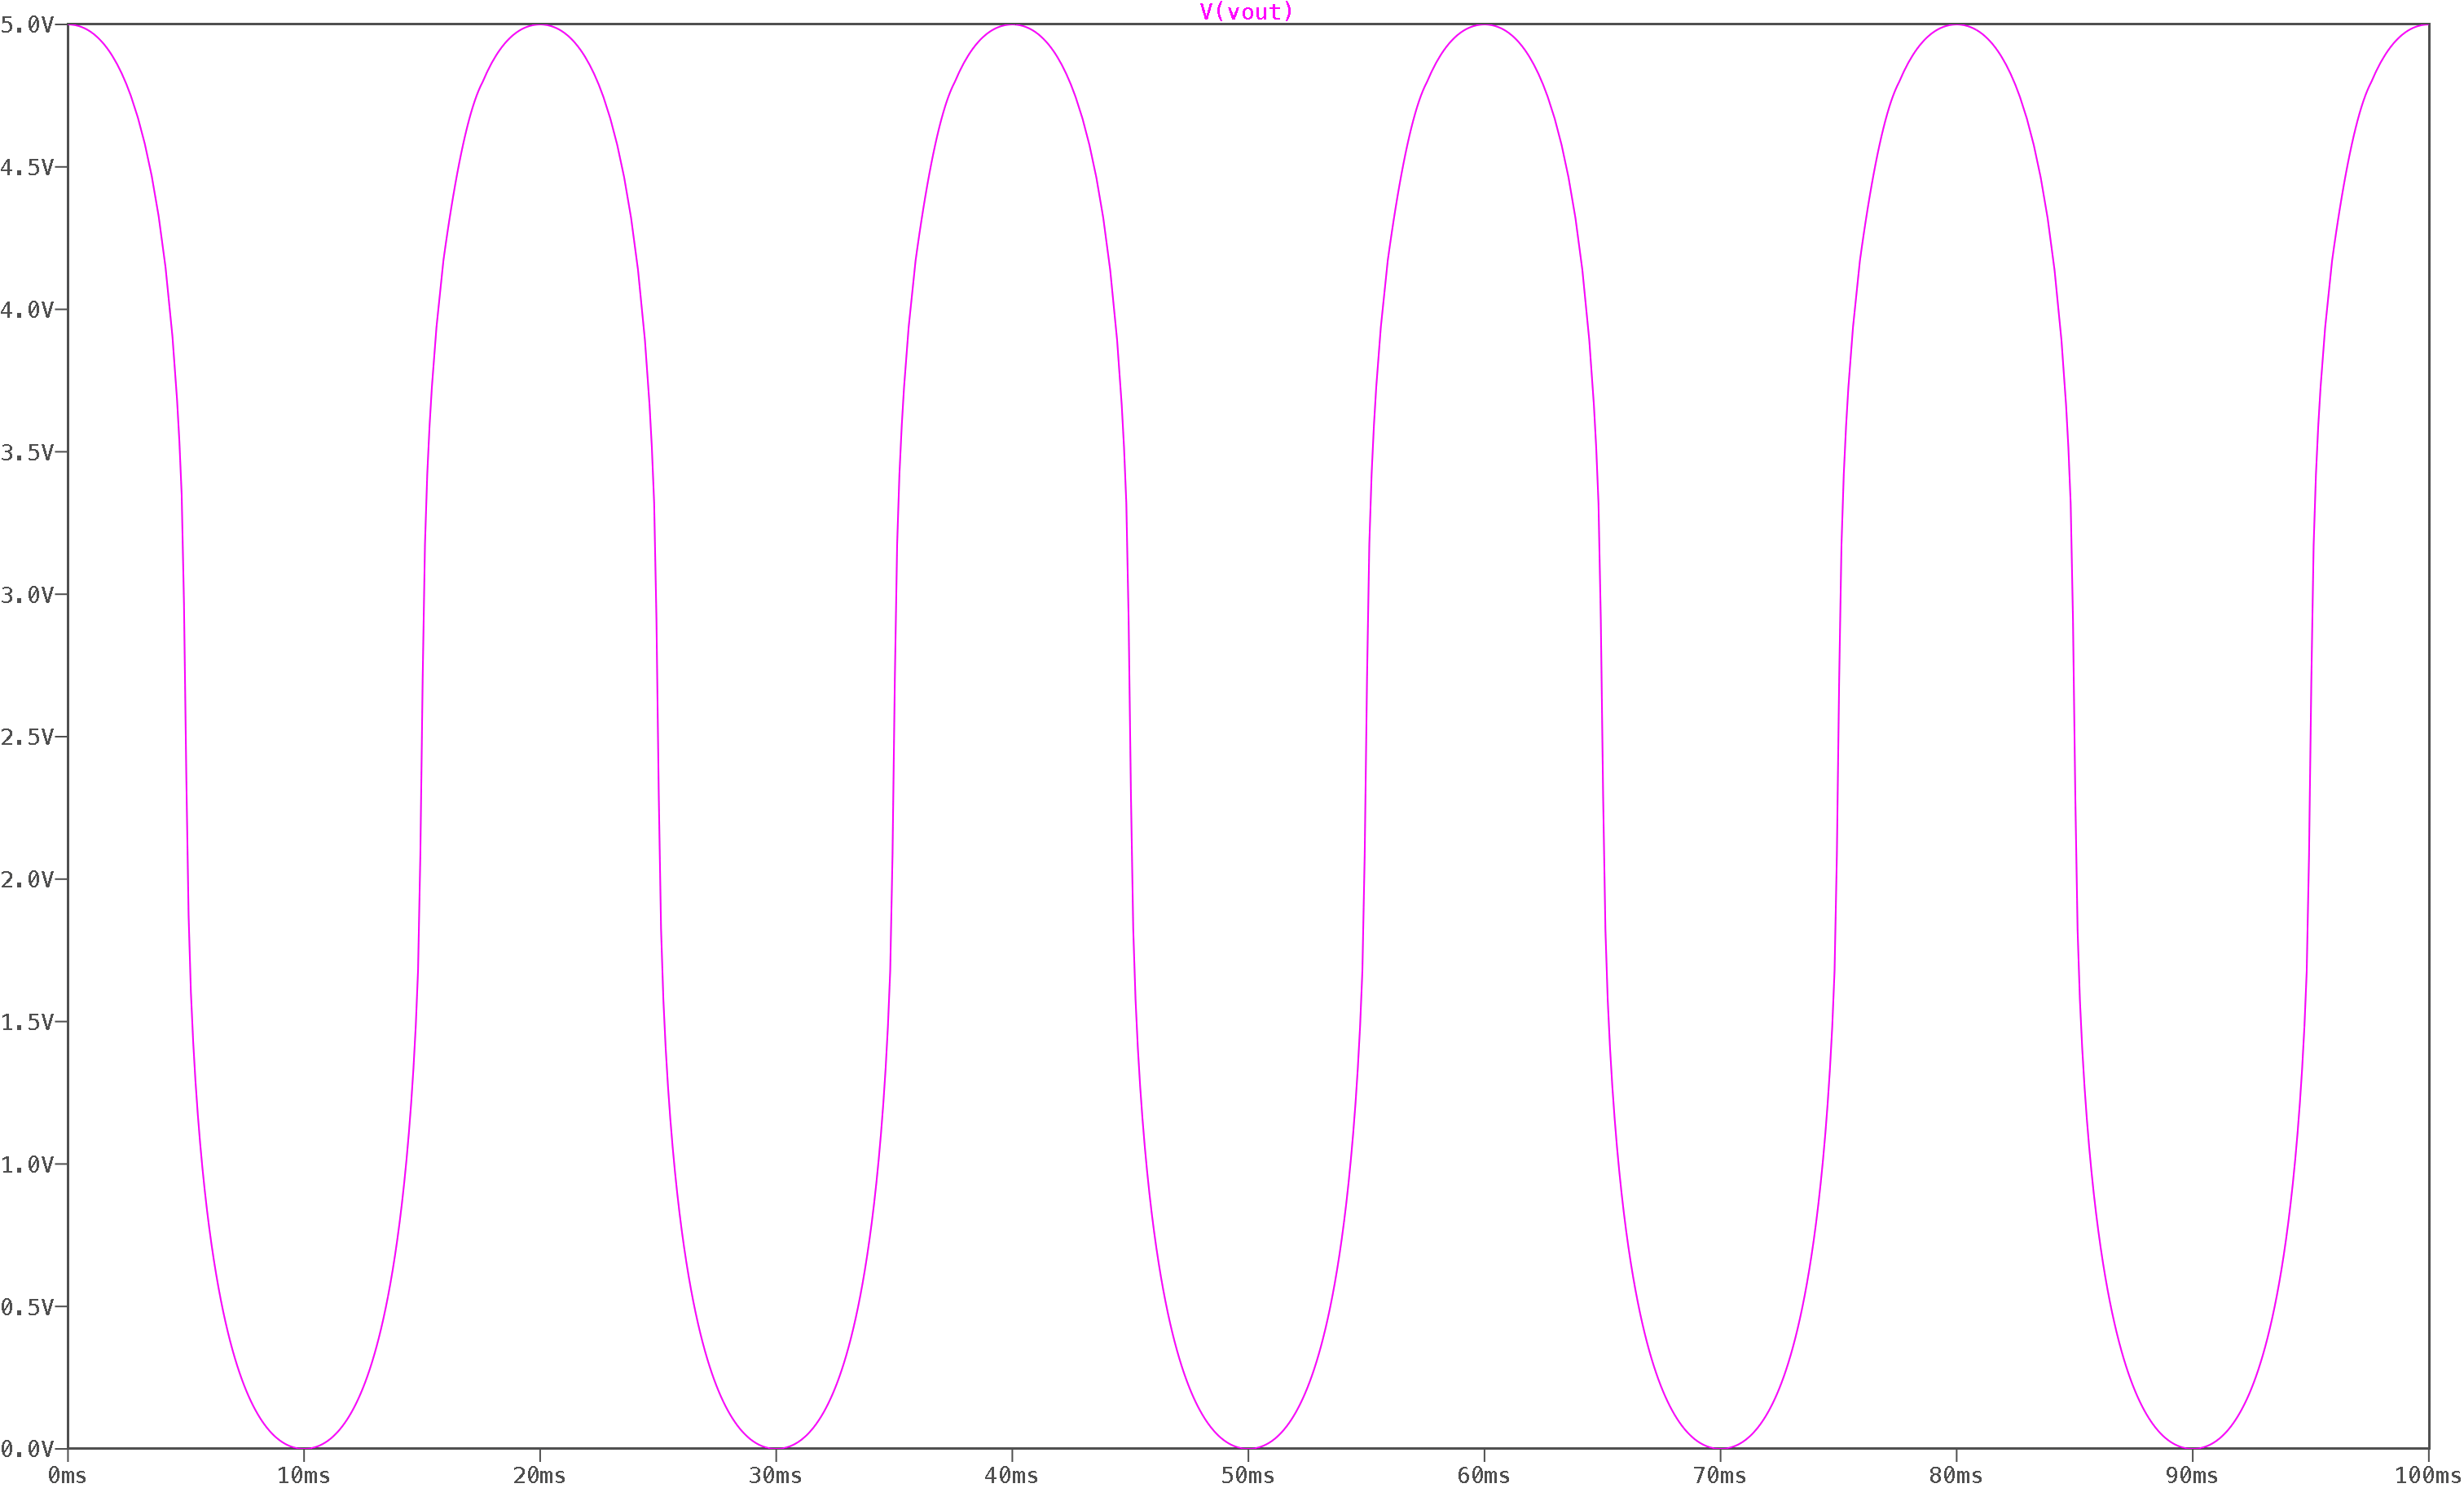
\includegraphics[width=1.0\columnwidth]{LTspice_CMOS_Inverter_graph.png}
    \caption{LTspice CMOS Inverter Circuit Graph}
    \label{fig:positive_clamper}
\end{figure}

\noindent{Now, when we give a square wave as input of same amplitude and offset and keep everything as it is we can study the characteristics of CMOS such as its rise time and fall time of output and calculate its delay of input and output.}

\begin{figure}[H]
    \centering
    \includegraphics[width=1.0\columnwidth]{Input and Output Square Waveform.png}
    \caption{CMOS Inverter Circuit Graph(Square Wave)}
    \label{fig:positive_clamper}
\end{figure}

\noindent{From this graph we can easily calculate rise time , Fall time and propogation delay low to high and high to low.}


\section{Discussion}
\noindent{CMOS Inverter has maximum rail to rail voltage  at output  as seen in VTC curve ,which implies that VLSI circuit with static CMOS logic design  gives high noise margin,low power dissipation and high fanout but same time used two transistor for a single input in cost of increases overall area and circuit with CMOS logic design becomes slower. The graph can be seen below:}


\section{Conclusion}
\noindent{The characterization of the CMOS inverter in this experiment highlights its fundamental operation and key performance metrics such as rise time, fall time, and propagation delay. The experimental results, verified through LTspice simulations, confirm the theoretical expectations of CMOS behavior, including its rail-to-rail output swing and transition characteristics. The voltage transfer characteristic (VTC) curve demonstrates the high gain in the switching region, validating the inverter’s role as a fundamental building block in digital logic design. Despite its advantages such as low power dissipation, high noise margin, and robust performance, the CMOS inverter’s requirement for both PMOS and NMOS transistors increases circuit complexity and area. Overall, the experiment successfully establishes the inverter’s essential properties, reinforcing its significance in VLSI circuit design.}



\begin{thebibliography}{00}
\bibitem{1}
Fundamentals of Microelectronics by Behzad Razavi
\bibitem{2}
 Microelectronic circuits by Adel Sedra and Kenneth Smith	
\end{thebibliography}

\end{document}
